\documentclass{standalone}
\usepackage{pgfplots}
\pgfplotsset{compat=1.18}
\usepgfplotslibrary{fillbetween}

\begin{document}

\definecolor{tab_blue}{HTML}{1F77B4}
\definecolor{tab_orange}{HTML}{FF7F0E}
\definecolor{tab_green}{HTML}{2CA02C}
\definecolor{tab_red}{HTML}{D62728}


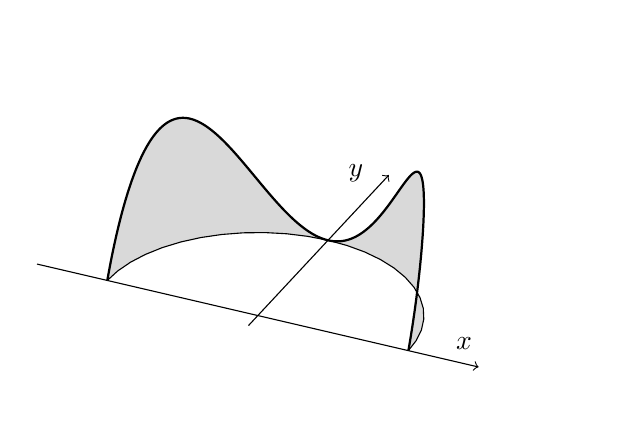
\begin{tikzpicture}[baseline]
\begin{axis}[
axis lines = middle,
unit vector ratio*=1 1 1,
scale=1.2, xmin=-2.2, xmax=2.2, ymin=-0.2, ymax=2.8, zmin = -0.2, zmax = 1.0,
hide z axis,
%grid = major,
view={25}{30},
ticks=none,
%xtick={0,1},
%ytick={0,1},
%ztick={0,1},
%xticklabels = {0,1},
%yticklabels = {0,1},
%zticklabels = {0,1},
xlabel=$x$,
ylabel=$y$,
%zlabel=$z$,
axis line style = {->},
]
\pgfmathsetmacro{\R}{1.5}
\pgfmathsetmacro{\a}{0}
\pgfmathsetmacro{\b}{pi}
\addplot3[samples=300, thick, samples y=0, domain=\a:\b, name path=up] ({\R*cos(deg(x))}, {\R*sin(deg(x))}, {(\R)^3*(cos(deg(x)))^2*sin(deg(x))});
\addplot3[samples y=0, domain=\a:\b, name path=down] ({\R*cos(deg(x))}, {\R*sin(deg(x))}, 0);
\addplot3[fill=gray!30] fill between [of=up and down]; 

\end{axis}
\end{tikzpicture}

\end{document}